 
% ME3001   
% Tristan Hill - Spring 2024 
% this assignment was adapted from matlab_workshop lab8
% graphics ans transformations


% Document setting
\documentclass[11pt]{article}
\usepackage[margin=1in]{geometry}
\usepackage[pdftex]{graphicx}
\usepackage{multirow}
\usepackage{setspace}
\usepackage{hyperref}
\usepackage{color,soul}
\usepackage{fancyvrb}
\usepackage{framed}
\usepackage{wasysym}
\usepackage{multicol}

\pagestyle{plain}
\setlength\parindent{0pt}


% assignment number 
\newcommand{\NUM}{6} 
\newcommand{\HSPC}{42mm} 
\newcommand{\HHSPC}{33mm} 
\newcommand{\VSpaceSize}{2mm} 
\newcommand{\HSpaceSize}{2mm} 

\definecolor{mygray}{rgb}{.6, .6, .6}

% [153,50,204] - dark orchid
\definecolor{mypurple}{rgb}{0.6,0.1961,0.8}
%[139,69,19] - saddle brown
\definecolor{mybrown}{rgb}{0.5451,0.2706,0.0745}


\begin{document}

	\textbf{\LARGE ME3001 - Spring 2024} \\\\
	\textbf{\LARGE Weekly Activity \NUM:  Using Two-Dimensional Arrays}\\\\
	\textbf{\LARGE Graphics - The Patch Object + Transformations} \\
	
	\begin{description}
        \vspace{5mm}
		\item [\textbf{ \Large Overview}] \textbf{ \Large :}\\
		
		You are going to practicing using two dimensional arrays in MATLAB. These are often referred to as Matrices and this is where MATLAB gets its name! There are many tools built in for working with matrices. If you are curious check the help. Today we are going to practice the basics and learn a new way to make graphics in MATLAB.

	    \item [\textbf{ \Large }] \textbf{ \Large Basic Form of a Matrix:}\\
	    
	    The {\bf size} of a matrix is the {\bf number of rows} and the  {\bf number of columns} in the matrix respectively. The matrix A shown below has m rows and n columns.
	    
\Large{
\[ A =\left( \begin{array}{cccc}
a_{11} & a_{12} & ...& a_{1n} \\
a_{21} & a_{22} & ...& a_{2n} \\
&.&&\\
&a_{ij}&&\\
&.&&\\
a_{m1} & a_{m2} & ...& a_{mn}\end{array} \right) \] }
		 
        \item [\textbf{ \Large }] \textbf{ \Large Initializing a Two Dimensional Matrix:}
		\begin{itemize}
	\item Choose a valid variable name and use the {\it square brackets} to create a matrix with hardcoded data.

	\item Commas (,) separate columns of the matrix. Spaces also work.

	\item Semicolons (;) separate rows of the matrix. A newline will also work.

\end{itemize}

	\item [\textbf{ \Large }] \textbf{ \Large Accessing and Assigning:}
		\begin{itemize}
		\item Basically the same as with 1D
		\item \scalebox{1}{{\fontfamily{qcr}\selectfont  x = A(3,5) \% access element in row 3 column 5}} 
		\item \scalebox{1}{{\fontfamily{qcr}\selectfont  y = 25) }} 
		\item \scalebox{1}{{\fontfamily{qcr}\selectfont  A(6,2) = y \% assign element in row 6 column 2}} 
		
		\end{itemize}
\newpage
    \item [\textbf{ \large Example}] \textbf{ \Large :}\\ \\  The program below generates figure1 shown on the next page using a patch object. \\
		
\scalebox{1}{{\fontfamily{qcr}\selectfont clear variables;clc;close all}}\\
\scalebox{1}{{\fontfamily{qcr}\selectfont s=1;}}\\
\scalebox{1}{{\fontfamily{qcr}\selectfont cube.vertices=[0, 0, 0 }}\\
\scalebox{1}{{\fontfamily{qcr}\selectfont \hspace{\HSPC}              s, 0, 0}}\\
\scalebox{1}{{\fontfamily{qcr}\selectfont \hspace{\HSPC}               s, s, 0}}\\
\scalebox{1}{{\fontfamily{qcr}\selectfont  \hspace{\HSPC}              0, s, 0}}\\
\scalebox{1}{{\fontfamily{qcr}\selectfont \hspace{\HSPC}              0, 0, s }}\\
 \scalebox{1}{{\fontfamily{qcr}\selectfont  \hspace{\HSPC}             s, 0, s }}\\
\scalebox{1}{{\fontfamily{qcr}\selectfont   \hspace{\HSPC}             s, s, s}}\\
\scalebox{1}{{\fontfamily{qcr}\selectfont  \hspace{\HSPC}             0, s, s];}}\\

\scalebox{1}{{\fontfamily{qcr}\selectfont cube.faces=[1, 2, 3, 4}}\\
\scalebox{1}{{\fontfamily{qcr}\selectfont   \hspace{\HHSPC}      5, 6, 7, 8}}\\
\scalebox{1}{{\fontfamily{qcr}\selectfont   \hspace{\HHSPC}          1, 2, 6, 5}}\\
\scalebox{1}{{\fontfamily{qcr}\selectfont    \hspace{\HHSPC}          2, 3, 7, 6}}\\
\scalebox{1}{{\fontfamily{qcr}\selectfont     \hspace{\HHSPC}         3, 4, 8, 7}}\\
 \scalebox{1}{{\fontfamily{qcr}\selectfont   \hspace{\HHSPC}          4, 1, 5, 8];}}\\

\scalebox{1}{{\fontfamily{qcr}\selectfont figure(1)}}\\
\scalebox{1}{{\fontfamily{qcr}\selectfont ph=patch(cube);}}\\
\scalebox{1}{{\fontfamily{qcr}\selectfont ph.EdgeColor=[1.0000,0.8667,0];}}\\
\scalebox{1}{{\fontfamily{qcr}\selectfont ph.FaceColor=[0.3098,0.1608,0.5176];}}\\
\scalebox{1}{{\fontfamily{qcr}\selectfont ph.LineWidth=2;}}\\
\scalebox{1}{{\fontfamily{qcr}\selectfont axis equal}}\\
\scalebox{1}{{\fontfamily{qcr}\selectfont view(3)}}\\
		
		\item 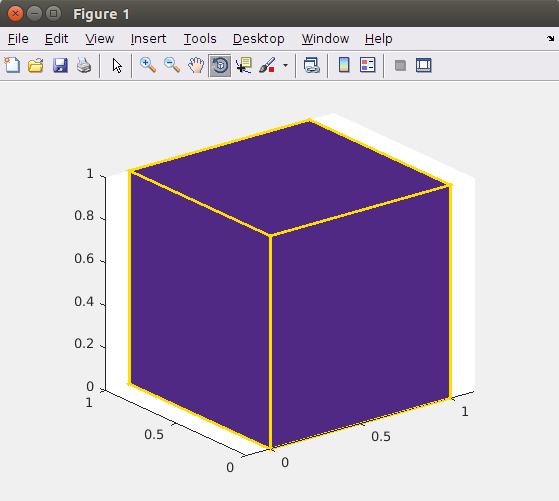
\includegraphics[scale=.8]{lab8_fig1.png}\\
      		\item 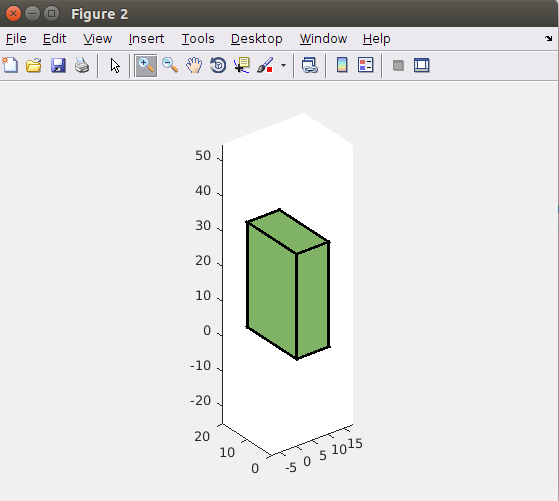
\includegraphics[scale=.8]{lab8_fig2.png}\\
      		\item 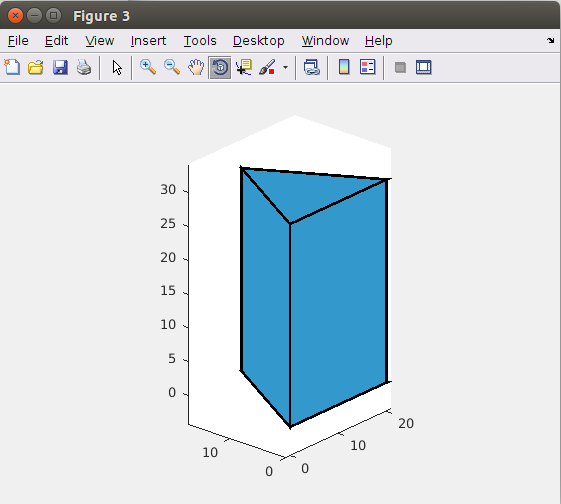
\includegraphics[scale=.8]{lab8_fig3.png}\\
      		\item 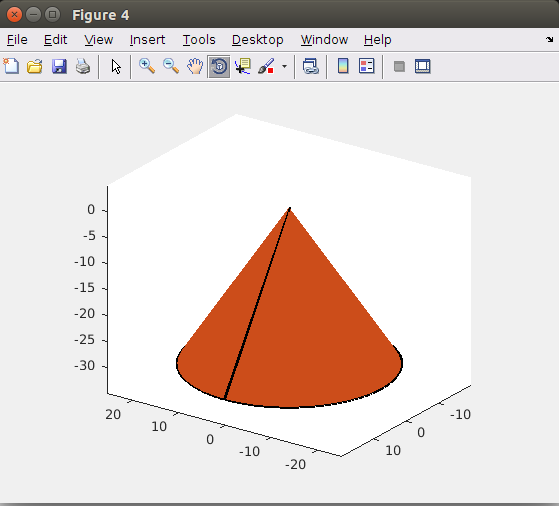
\includegraphics[scale=.8]{lab8_fig4.png}
	 
  \item [\textbf{ \large Assignment}] \textbf{ \Large :}\\

  \begin{enumerate}

    \item Generate a 3D object using the patch command. Use one of the examples shown or create your own.

    \item Adjust the lighting and other properties by setting the patch parameters.

    \item Choose a direction and distance and translate the object using a matrix operation.

    \item Choose an axis and angle and rotate the points about that axis using a rotation matrix.

    \item ...

  \end{enumerate}

  \item [\textbf{ \large Deliverables}] \textbf{ \Large :}\\
  \begin{itemize} 
   \item Submit working MATLAB code as a .m file which demonstrates all numbered assigment parts.

   \item Include at least two images of the object you have created from different viewpoint. They can be in a .pdf, .docx, or attached directly to the assignment in standard image format (.png, .jpg),

  \end{itemize}
  \end{description}
 
\end{document}



